\section{Chapter 3 -- fMRI analyses} % (fold)
\label{sec:task_and_models}
This chapter has 4 parts, all address different aspects of fMRI data collection and analysis.  First is the methodological details of the fMRI functional (i.e., BOLD) and structural acquisition, as well as the preprocessing of that data.  Little here exceeds or differs from current accepted fMRI data practices \citep{Poldrack:2008p6570,Amaro:2006p2638,Bullmore:1996p6538}.  Second null-hypothesis test thresholded maps of BOLD activity are considered (i.e. whole-brain patterns of activity are discussed).  The third section describes an alternative to the whole-brain analysis, focus on comparing BOLD time-courses from anatomical regions of interest to the reinforcement learning models from the previous chapter (p\pageref{sub:threemodels}).  In this, the focus is on ranking models using information theory metrics, not trying to select \emph{a} correct model as one might do in more traditional ROI analyses (for example, \citet{Poldrack:2006p9841,Mars:2010p7999}).  Fourth is the results from the region of interest analyses described in part three.  These results are, in general, highly supportive of rewards as categories, though the argument for that conclusion is held off until the next, final, chapter (p\pageref{sec:dicussion}).

\subsection{An Acquisition}
\label{sub:acquired}
\subsubsection{Data details}
\label{subsub:datadetails}
fMRI data was acquired at the Intermountain Neuroimaging Consortium (INC) facility located at the University of Colorado at Boulder on a Siemens Allegra 3T (whole body) scanner.  All 18 right-handed participants were pre-screened for the typical fMRI exclusion factors (e.g., metal implants, mental disorders, etc).  High resolution anatomical data was acquired as a T1-weighted structural image, MPRAGE sequence, at 1x1x1 mm, (256 x 156 x 192) with a TR of 2530 ms, and TE of 1.64 ms, with a flip angle of 7$^\circ$.  All functional (i.e., BOLD) data was acquired with T2-weighted echo-planar imaging (EPI), at 2.29 x 2.29 x 4.00 mm (96 x 96 x 26), with a TR of 1500 ms, a TE a 25 ms, a flip angle of 75$^\circ$ and a FOV of 220 mm.

Four sets of functional data were acquired.  The first was of the ``refresher'' for part 1 of the behavioral training (p\pageref{subsub:whatwhen}), spanning 241 volumes.  The second and third spanned part 2 of the stimulus-responses learning task, divided into 2 (nearly) even sets lasting 390 and 394 volumes respectively (again see p\pageref{subsub:whatwhen}).  The fourth scan featured repeated presentation of gratings from both reward categories, in a random order.  The intent of this scan was to isolate rewarding activity outside the primary task. This localizer was not in the end useful (discussed on p\pageref{subsub:chunks}).

\subsubsection{Preprocessed (model) food}
\label{subsub:preprocessed}
Following DICOM to nifiti-1 conversion using dicom2nii (\url{http://www.mccauslandcenter.sc.edu/mricro/mricron/dcm2nii.html}), each dataset was subjected to the following preprocessing pipeline carried out in SPM8's batch mode (\url{http://www.fil.ion.ucl.ac.uk/spm/software/spm8/}).  For complete code see, \url{https://github.com/andsoandso/fmri/tree/master/catreward/spm\_m}.  Anatomical data was first segmented into white and grey matter regions \citep{Collignon:1995p9347}.  Based on these segments the parameters necessary for normalization into a standard reference space (T1 MNI-352, at 1 mm, MNI space or short) were calculated. Normalization had two steps.  The first was a Bayesian 12-parameter affine transformation \citep{Ashburner:1997p9348}.  The second was a set of nonlinear deformations, using a 1127 parameter discrete cosine transform \citep{Ashburner:1999p9350}.  Anatomical data was then resampled from 1.27 to 1.00 $mm^3$ using fourth degree $\beta$-splines, and finally, using the parameters above, normalized into MNI space.

To correct for the slight head movements that often occur during scanning, movement regressors for all volumes of the functional data were first calculated \citep{Ashburner:1999p9350}.  No participant moved more than 1.5 mm, so all data was retained.  Functional data was then slice-time corrected, using slice 13 (the middle slice from the descending acquisition) as the reference, followed by coregisteration with the pre-processed (native-space) anatomical data, and resampling into 3 mm$^3$ voxels, again using fourth degree $\beta$-splines \citep{Collignon:1995p9347}.  Functional data was then normalized into MNI space using the anatomically-derived parameters above.  Finally, the functional data was spatially smoothed using a 6 mm FWHM Gaussian, though a copy of the unsmoothed data was retained for the ROI analyses (described on p\pageref{sub:regoins}).  Just prior to regression analysis, each voxel's time course was also low-pass filtered using finite impulse response model, with a cutoff at 0.008 Hz \citep{Kruggel:1999p9351}.  For all whole-brain analyses, the movement regressors were entered into the regression models as covariates, accounting for any head movement.  Given the large spatial averages employed in the ROI analyses these weren't motion corrected \citep{Poldrack:2007p8572}.

\subsubsection{The best of all possible signals}
\label{subsub:bestsignal}
In fMRI, and in general time-series analysis, there is an intrinsic trade-off between detecting a signal in the presence of noise and estimating the shape of that signal \citep{Dale:1999p7901,Birn:2002p1777,Liu:2004p2141}.   One way to optimize over both these conflicting objectives is to manipulate the trial order in a rapid event-related design \citep{Miezin:2000p7924}.  One state-of-the-art method for optimizing the trial ordering process is a genetic algorithm which uses two (weighted) loss functions, one for signal detection and one for time-course estimation \citep{Wager:2003p2980}. \citet{Kao:2009p7899}, improved on Wager's (2003) initial design by adding in a loss function for psychological considerations, greatly improving execution speed and documentation.  As a result, Kao et al's (2009) method/code was used to optimize trial orders for part 1 and 2 of the behavioral task (p\pageref{subsub:whatwhen}), along with the reward category localizer scan (p\pageref{subsub:datadetails}).

\subsection{Mobs of Blobs}
\label{sub:blob}
All statistical parametric maps (below) were derived from a Random Effects analysis (RFX, or ``second-level'' in SPM8 jargon), multiple comparison corrected assuming Gaussian Random Fields using the Family Wise Error Rate (FWE) at the $p < 0.05$ level, with a minimum cluster size of 4 voxels \citep{Worsley:1996p9367}. 

Whole brain activity for the stimulus-response learning portion of the behavioral experiment (i.e., part 2, p\pageref{subsub:whatwhen}) was examined first by comparing all trials to the baseline (rest) condition.  This data is presented in two ways. First is the statistical thresholded image.  This contrast map showed significant bilateral activity in the cerebellum, insula and anterior cingulate ($t$(15) = 6.59, $p< 0.05$; Figure~\ref{fig:gl}).  Second is an overlay of the raw $t$-values, which allows for visual confirmation the observed significant effects were robust and widespread in their respective regions, but also allowed for the analysis of overall and sub-threshold patterns of activity.  These raw data suggested near threshold levels of activity in the head of the caudate, ventromedial, dorsolateral frontal cortices as well as (weaker) activity in the occipital lobe (Figure~\ref{fig:glraw}).  And indeed in a two-way ANOVA looking at that interaction between gains and losses, significant clusters were observed in head and body of caudate, insula, posterior and anterior cingulate with the posterior activation extending into the precuneus, as well as in dorsolateral (i.e middle frontal) PFC, and in ventrolateral PFC (Figure~\ref{fig:gxl}; $F$(1, 270) = 30.76, $p < 0.05$).  When gains and losses were examined separately, but again compared to rest, both had activity in the same areas as in the combined condition (not shown).

\begin{figure}[tp]
    \noindent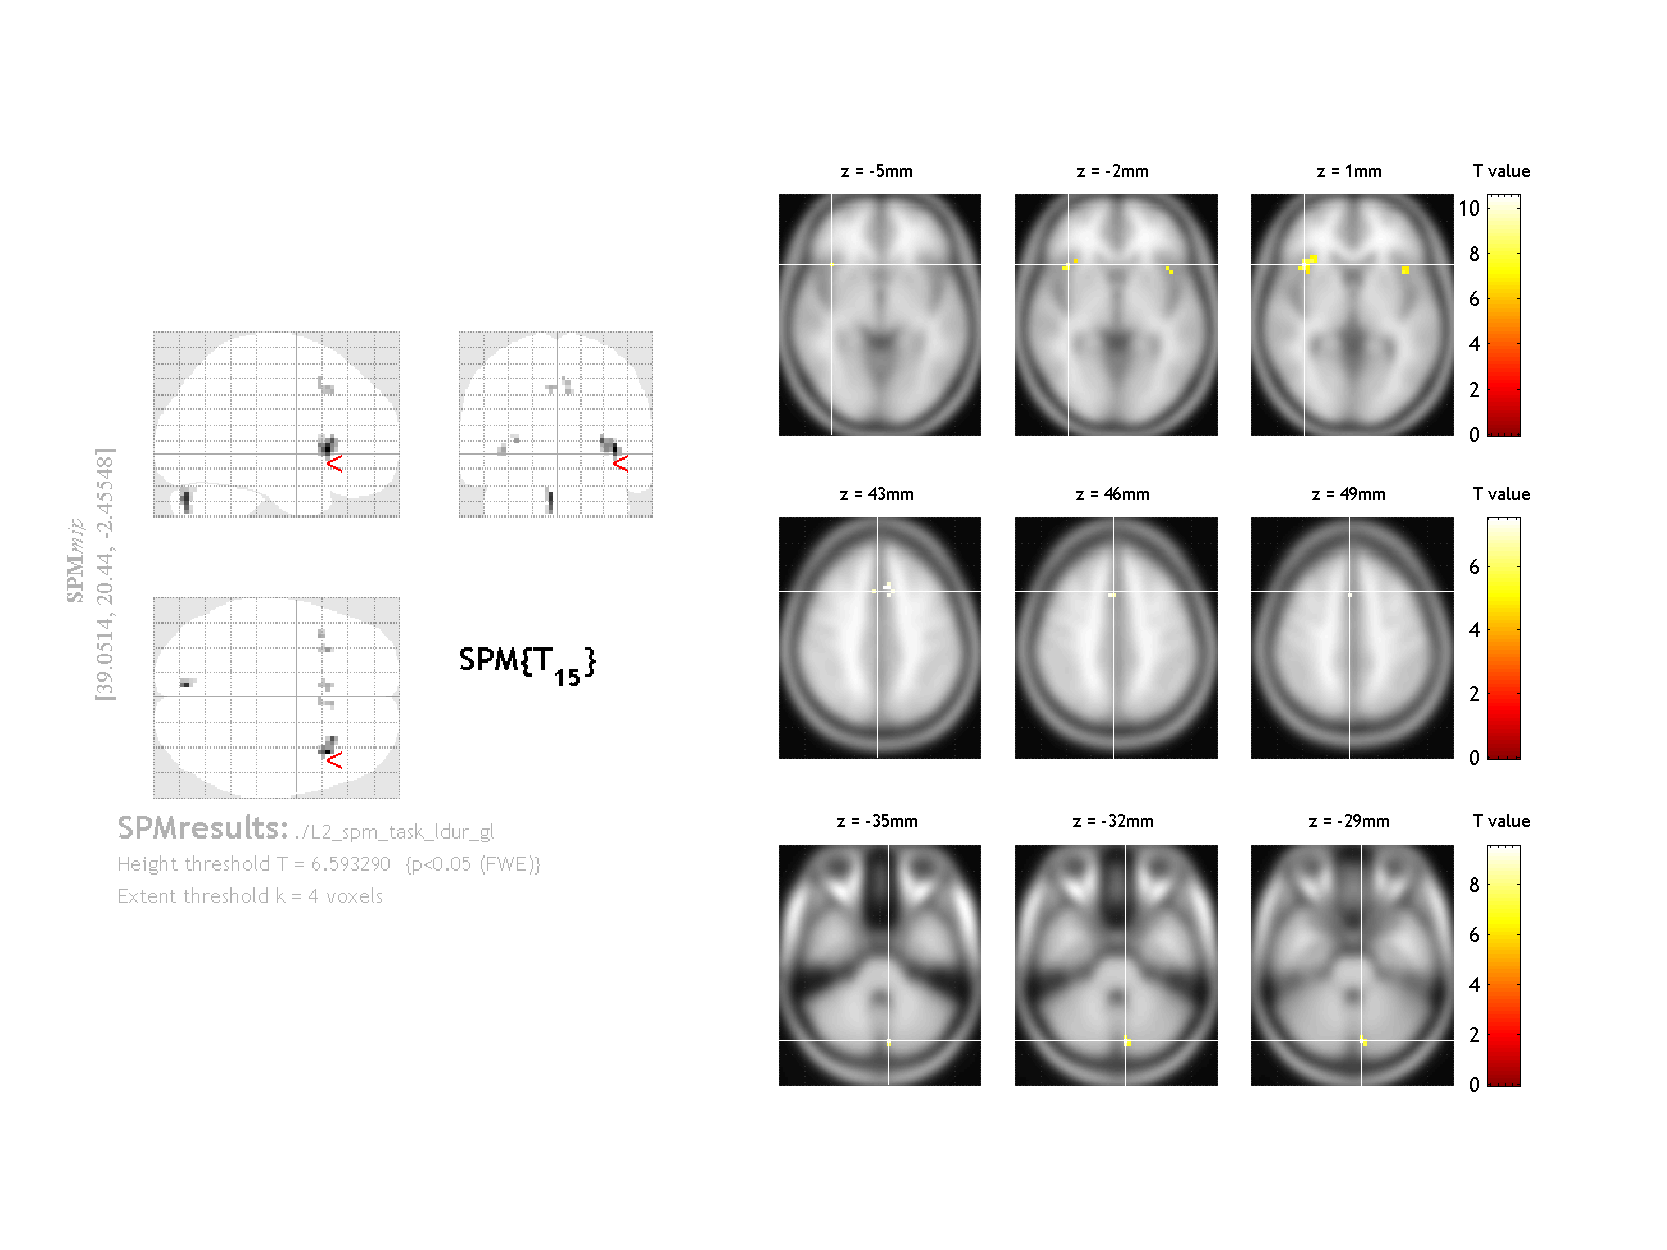
\includegraphics[width=39pc]{f_map_gl_p05}
    \centering
    \caption{Statistical parametric map for all trials in the stimulus-response learning task (i.e., part 2, p\pageref{subsub:whatwhen}), compared to the rest period.  \emph{Left} is a glass brain, showing all significant clusters.  \emph{Right} is a set of axial slices highlighting strong areas of activity overlaid onto the T1 MNI-352 template.  $Z$ is the height of the axial slice in MNI space.}
    \label{fig:gl}
\end{figure}

\begin{figure}[tp]
    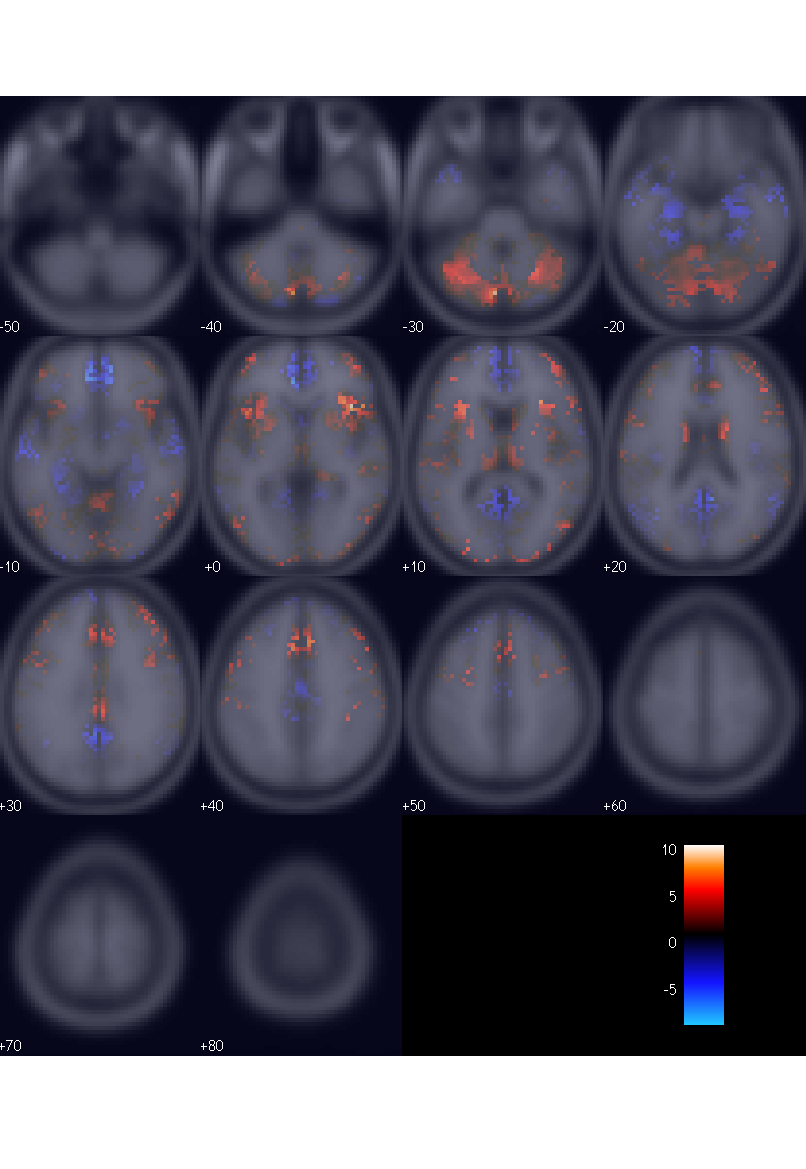
\includegraphics{f_map_gl_raw_t}
    \centering
    \caption{The $t$-values for all trials in the stimulus-response learning task (i.e., part 2), compared to the rest period,  overlaid onto the T1 MNI-352 template.   Each number is the height of the axial slice in MNI space.}
    \label{fig:glraw}
\end{figure}

\begin{figure}[tp]
    \noindent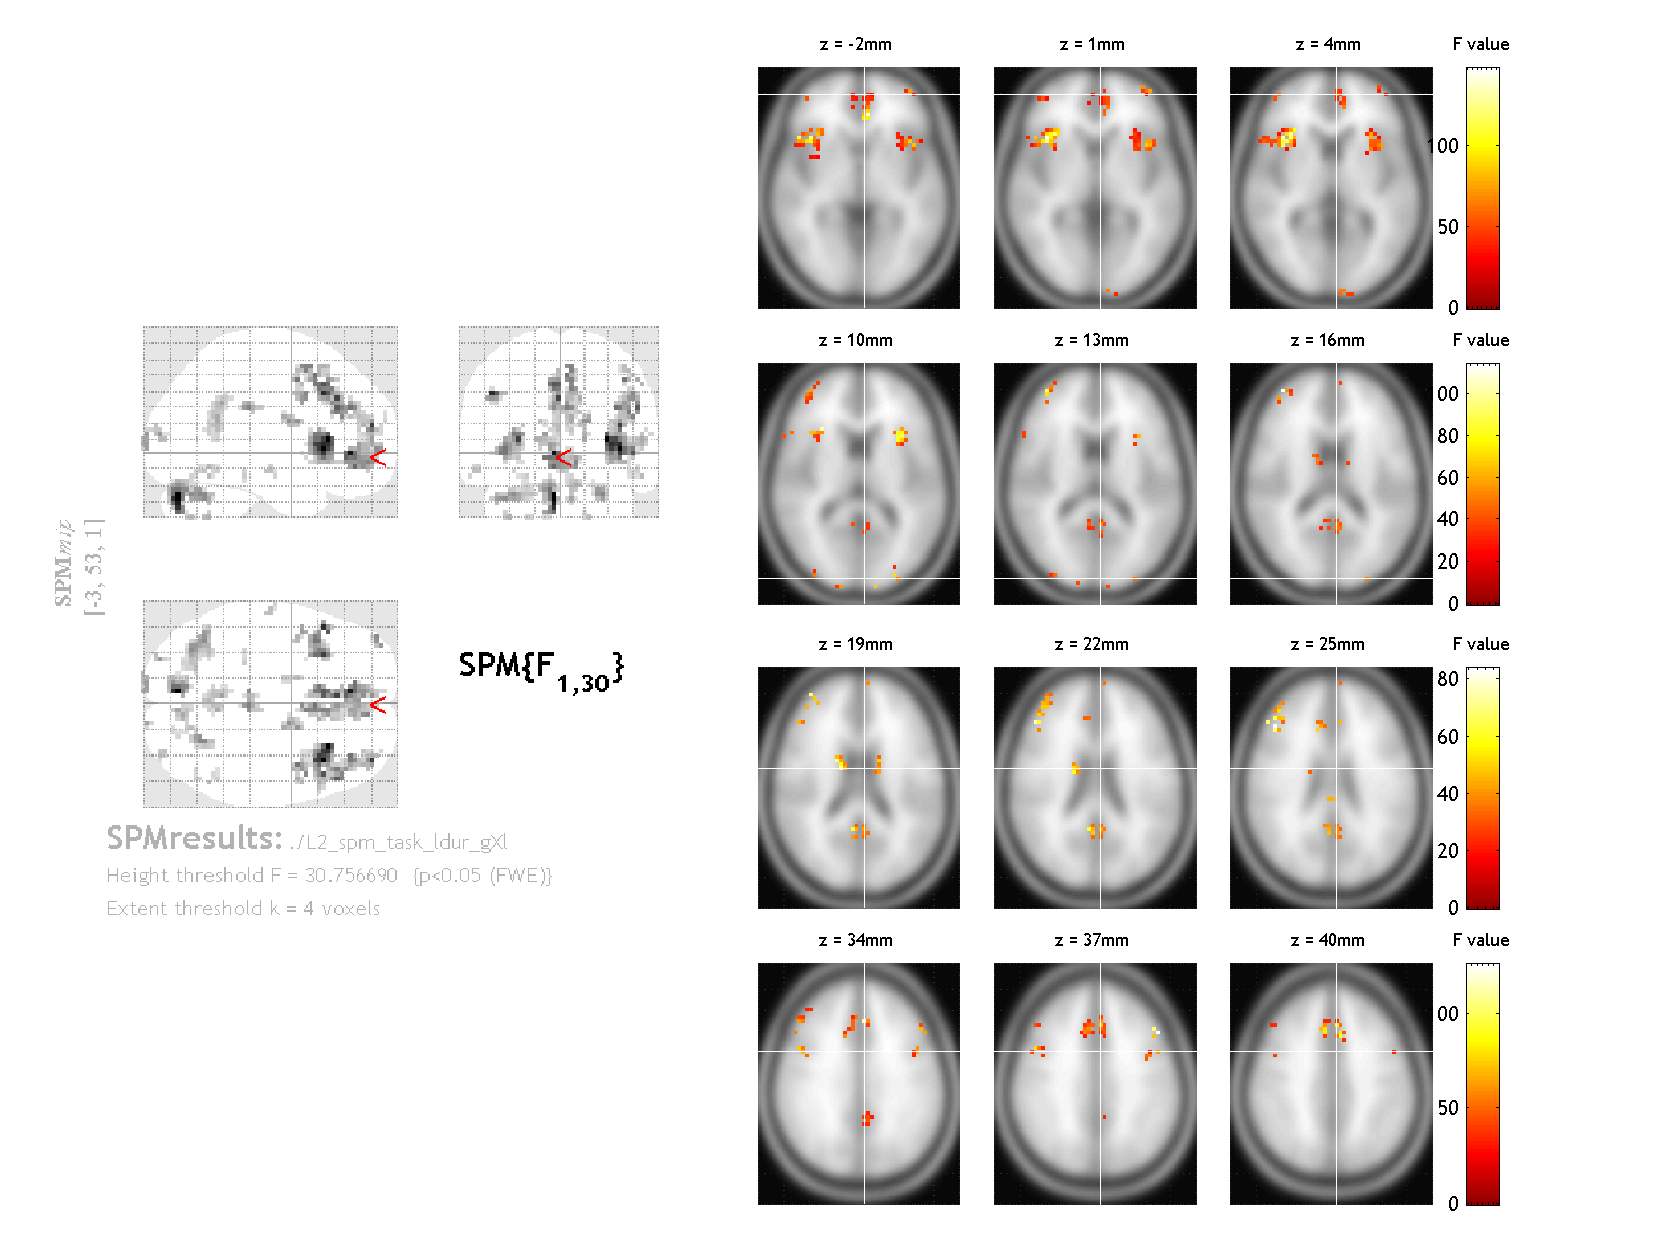
\includegraphics[width=39pc]{f_map_gxl_p05}
    \centering
    \caption{Statistical parametric map for all trials in the stimulus-response learning task (i.e., part 2) examining the interaction between gains and losses.  \emph{Left} is a glass brain, showing all significant clusters.  \emph{Right} is a set of axial slices highlighting strong areas of activity overlaid onto the T1 MNI-352 template.  $Z$ is the height of the axial slice in MNI space.}
    \label{fig:gxl}
\end{figure}

\subsection{Regions and Models}
\label{sub:regoins}
\subsubsection{The right chunks}
\label{subsub:chunks}
Following whole-brain analysis, regions of interest were selected using two separate yet related methods.  The first employed only regions from the Harvard-Oxford probabilistic anatomical atlas, using the 50\% cutoff \citep{Desikan:2006p9370}.  The second combined anatomical regions with functional clusters isolated using both the data collected during the second half of part 1 (i.e., the ``refresher'') and from the reward category localizer (p\pageref{subsub:datadetails}).  Comparisons between them showed the anatomically-limited functional clusters and the entire anatomical regions displayed very similar results.  So to limit the complexity of later analyses, and to increase power, functional clusters were discarded in favor of the larger anatomical regions.  Most anatomical regions of interest were selected \emph{a priori} based on previous studies of reinforcement and category learning (see the \emph{Introduction} for a review).  Left and right subcortical regions of interest were the dorsal caudate, ventral striatum/nucleus accumbens, and putamen.   Bilateral cortical areas were the middle frontal cortex (i.e., dorsolateral PFC), frontal medial cortex (which contains ventrolateral PFC), and orbital frontal cortex.  Based on the whole-brain maps (p\pageref{sub:blob}), regions for the insula, anterior and posterior cingulate (ACC and PCC for short) were included as well. While these is no strong \emph{a priori} hypothesis for the role of these regions may play or may not play, activity in each of these \emph{post hoc} regions is common to human category learning experiments \citep{LopezPaniagua:2011p8296,Seger:2010p7188,Cincotta:2007p6672,Seger:2006p5447,Seger:2005pd}.


% -- PROOFED ABOVE
\subsubsection{A way to(o) many}
\label{subsub:tomany}
There are 6 models under evaluation: the three kinds of similarity adjustment (``none'', ``exp'', and ``gauss'') multiplied by the two possible reward codes (``acc'' and ``gl''), with the two terms of interest (i.e., value and the reward prediction error), that is 12 comparisons.  The were also a number of \emph{a priori} confounds to the signals of interest including the similarity metrics, the reward codes, and the grating parameters, bringing the total to 23.  As the models are not nested\footnote{
    Often defined by whether or not two models can be made identical by adding or subtracting parameters \citep{Forster:2000p9623}} and therefore not amenable to $F$-tests -- the common statistical way to compare model fits -- an alternative approach was called for.  Further complicating the issue was the fact that each of the models is covariate, if not collinear, with the others.  To top it off, none of the three similarity-adjustments are statistically independent; reinforcement learning can be viewed as a regression of the reward code onto behavioral choices.  All these factors combined would make statistical testing difficult, to say the least.  But fortunately finding \emph{the} best model is not the goal.  

The latest recordings of phasic (i.e., reward prediction) activity in the VTA/SNc suggests a complicated reward and prediction error coding scheme (see p\pageref{subsub:expectations}), wherein several separate sets of calculations may be carried out independently \citep{Kim:2006p1063, Matsumoto:2009p7219, Smith:2011p8133}.  The observed BOLD signal is then an aggregate of these many activities. It is possible, even likely, then that more than one of the models is correct making null hypothesis tests an incorrect choice.  Model selection is the right choice.

Model selection is the process of finding a \emph{family} of models that best predict a given dataset \citep{Rao:2001p9457}.  Most techniques try to wisely balance parsimony with increasing fit (i.e., solving the bias versus variance dilemma \citep{Geman:1992p9469}).  Unfortunately most model selection techniques require assumptions the models cannot meet (e.g., statistical independence).  The few that can tend to be complex recent statistical inventions.  Rather than navigate those troubled and unproven waters, a simpler approach was taken. Each model was independently examined and ranked, in an approach loosely similar to model averaging \citep{Forster:2000p9623}.

An AIC score (Akaike Information Criterion \citep{Akaike:1974p9530}) was assigned to each of the models/codes for every participant and region of interest.  The absolute AIC score across participants is not however meaningful.  Only the relative values are of interest \citep{Wagenmakers:2004p9472}.  As a result, individual's scores were normalized and ranked by subtracting the best (lowest) score from each \citep{Anderson:2000p9475}. The normalized set was then transformed to Akaike Weights, a way to easily compare the conditional probabilities of each model being true \citep{Wagenmakers:2004p9472}.  The Akaike Weights were then averaged across participants for each model and region of interest.

\subsubsection{Information on information}
\label{subsub:way}
AIC is a measure of loss; how much information is lost by substituting the model for the true distribution, i.e., the data.  The lower the AIC score, the better the model.  Unlike null hypothesis tests and Bayesian measures, AIC-based methods do not seek to find \emph{a} truth, but instead serve to rank models.  AIC offers then only relative insight, and is unable to make any claims about absolute significance.  Significance is a separate question, one to be returned to later.  Besides this limitation, AIC has some substantial advantages. Five are reviewed below.

One, unlike maximum-likelihood, AIC is designed to be a parsimonious score.  It penalizes for additional parameters.  It may therefore choose a worse model (as measured by likelihood or mean squared error) over a better but more complex one. This is the essence of Occam's razor\footnote{Famously and pithily expressed as, ``Entities are not to be multiplied beyond necessity''.}. 

Two, it fits with the process of science.  When designing an experiment it is rare that there are only two possible outcomes, instead typically there are several competing hypothesis, some of which may not be mutually exclusive.  AIC's focus on relative differences and evidential weights meshes perfectly with the reality of multiple working hypotheses \citep{Burnham:2004p9621}.

Three, truth can remain elusive.  A common alternative to AIC is BIC, the Bayesian Information Criterion.  Like AIC, BIC is derived from the log-likelihood of a model, however its derivation requires a rather strict (and often unrealistic) assumption -- that the true model is among the candidates \citep{Forster:2000p9623}.  And while it may be philosophically debatable whether any mathematical model can \emph{completely} describe reality, in this study the models are incomplete.  As, one, the human reinforcement learning literature contains several recent theoretically unaccounted for findings and, two, there are theoretical developments not included here to keep the models tractable.  

Four, AIC values are easily interpretable once they're transformed to Akaike Likelihoods or Weights\footnote{
    Likelihood for model $k$ among $K$ working hypotheses/models is given by $L_k = e^{-0.5({AIC}_k - {min}_{K}{(AIC)})}$, which is then normalized, becoming an Akaike Weight by $w_k = L_k / \sum\limits_{k=1}^K L_k$ \citep{Burnham:2004p9621}.}.  The likelihood is, as you would expect, simply the likelihood the model is correct (based on the information loss associated with it), while the Akaike Weights are normalized likelihoods.  As the Weights sum to one, the conditional likelihood of one model compared to another is just the ratio of their weights \citep{Burnham:2004p9621}.  For example, the conditional likelihood of model A over model B is just $w_A/w_B$.  That is, the likelihoods and Akaike Weights are intrinsically measures of effect size \citep{Anderson:2000p9475,Forster:2000p9623}.  Despite the fact that it is often used to express the likelihood of correctly rejecting the null hypothesis, the $p$ value is not a measure of effect, as $p$ is contingent not just on effect size but on sample number.  
    
    Five, AIC has a history with models of categorization. \citet{McKinley:1996p9532,Maddox:2001p9533}, among several others, used AIC to compare behavioral results to several alternative models of categorization.
    
\subsubsection{F-them}
\label{subsub:F}
AIC ranks offer no information about significance, in the familiar null hypothesis sense, or about the absolute fit of the model.  Both of these were addressed in a series of $F$-tests run prior to AIC analysis.  These (fixed-effect, across participant) omnibus tests asked whether the total set of regression parameters for each linear model (described below) could explain the BOLD time series better than chance (i.e could the null hypothesis (of 0) be rejected).  Keeping with recommendations of \citet{Burnham:2004p9621} and  \citet{Forster:2000p9623}, who argue that as AIC and significance tests are so dissimilar that direct comparison/interaction between them will be at best misleading, the models are not discarded based on significance.  All models are retained, and later AIC ranked.  The $F$-tests are a separate measure whose results are integrated during interpretation, not during model selection.

As is discussed in the results (for example see p\pageref{subsub:belowctx}), many of the models are significant by these omnibus $F$-tests, which might at first be rather shocking.  Many of the models and other regressors, including the simplistic ``boxcar'', make very different predictions about the BOLD response.  One would, therefore, expect only a few to be significant.  However this intuitive prediction is false, as each predictor is convolved with a haemodynamic response function which spans more than 20 seconds (p\pageref{sub:cmb}).  As a result, each single time point prediction is ``smeared'' across that temporal distance.   Unpublished Monte-Carlo simulations on the effect of this ``smearing'', confirm that null hypothesis tests, such as the $F$-tests here, are a poor metric of model quality and specificity, i.e., the likelihood the true model will be picked over some (related) alternatives.

\subsubsection{Code, BOLD, and models.}
\label{sub:cmb}
A total of 23 models were compared for each of the 12 regions of interest for each of the 16 subjects, 4416 comparisons in total.  Each of the models is described below (Table 1).  In general, a time-series (e.g the reward prediction error for each trial or the similarity for that trial's outcome) was convolved with a ``canonical''  haemodynamic response function, a mixture of gamma functions that serves as a parsimonious estimate of the (instantaneous) BOLD response \citep{Friston:1998p2022}.  The convolved series was then low-pass filtered, matching the treatment of the BOLD data (p\pageref{subsub:preprocessed}).  Each convolved and filtered model was then regressed onto the BOLD response for each participant's region of interest, retaining all parameters and fit measures inside subject-level HDF5 files.  The HDF5 format offers high performance read/write operations, and widespread support across several scientific programming languages (\url{http://www.hdfgroup.org/HDF5/}).

No available fMRI analysis package returns AIC scores (or measures that could be converted to such) and none allow for the efficient (i.e programmatic) analysis of many competing computational models. So a region of interest focused fMRI analysis tool was created in Python (v2.7.1) to meet those two needs.  This module, simply named ``roi'', has since been released under the BSD license and is available for download at \url{https://github.com/andsoandso/roi}. It relies on the nibabel library to read the nifiti-1 files  (v1.2.0; \url{http://nipy.org/nibabel}), nitime for time-series analysis, (v0.4; \url{http://nipy.sourceforge.net/nitime/}) Numpy for generic numerical work (v1.6.1; \url{http://numpy.scipy.org/}), with the GLS function from the scikits.statsmodels module handling the regressions (v0.40; \url{http://statsmodels.sourceforge.net/}).  Model-to-BOLD fit parameters, as well as other useful metadata, was then extracted and stored in text files suitable for importing into R (v2.15.1; \url{http://www.r-project.org/}).  All plotting and model ranking (as well as the $F$-tests) were carried out in R.  For complete BSD licensed code see, \url{https://github.com/andsoandso/fmri/tree/master/catreward/roi/results}.

\subsubsection{Our kinds of models}
\label{subsub:ourkinds}
To ease visualization and analysis each of the models was classified into one of 5 families.  Family one, denoted ``boxcar'', was identical to that first used in the whole-brain analysis (p\pageref{sub:blob}) -- all trials versus the rest condition.  This is a univariate time-series that predicts no trial-specific effects, i.e. no matter the task the brain, thus the BOLD response, just flicks on then off.  It serves as a useful standard against which to compare the model-based regressors.  The next two families were controls (i.e., \emph{a priori} covariates). The reward codes, both raw and similarity adjusted, were in one family (``control\_reward'') and in the other were the similarity metrics and grating parameters (``control\_similarity'').  The fourth family contained all the reward prediction errors (``rpe'').  The fifth contained all value estimates (``value'').

\newpage
\begin{center}
    \begin{longtable}{ | l | l | l | p{6cm} |}
    \caption{All models, their designations (Codes), families, and descriptions.}\\
    \hline
    Number & Code & Family & Description \\ \hline
         1 & 0\_1 & boxcar & The simplest model, a univariate analysis of all conditions. \\ \hline
         2 & acc & control\_reward & Behavioral accuracy. \\ \hline
         3 & acc\_exp & control\_reward & Behavioral accuracy, diminished by (exponential) similarity. \\ \hline
         4 & acc\_gauss & control\_reward & Behavioral accuracy, diminished by (Gaussian) similarity. \\ \hline
         5 & gl & control\_reward & Gains and losses. \\ \hline 
         6 & gl\_exp & control\_reward & Gains and losses, diminished by (exponential) similarity. \\ \hline
         7 & gl\_gauss & control\_reward & Gains and losses, diminished by (Gaussian) similarity. \\ \hline
         8 & rpe\_acc & rpe & Reward prediction error - derived from accuracy. \\ \hline
         9 & rpe\_acc\_exp & rpe & Reward prediction error - derived from accuracy diminished by (exponential) similarity. \\ \hline
        10 & rpe\_acc\_gauss & rpe & Reward prediction error - derived from accuracy diminished by (Gaussian) similarity. \\ \hline
        11 & value\_acc & value & Value - derived from accuracy. \\ \hline
        12 & value\_acc\_exp & value & Value - derived from accuracy diminished by (exponential) similarity. \\ \hline
        13 & value\_acc\_gauss & value & Value - derived from accuracy diminished by (Gaussian) similarity. \\ \hline
        14 & rpe\_gl & rpe & Reward prediction error - derived from gains and loses. \\ \hline
        15 & rpe\_gl\_exp & rpe & Reward prediction error - derived from gains and losses diminished by (exponential) similarity. \\ \hline
        16 & rpe\_gl\_gauss & rpe & Reward prediction error - derived from gains and losses diminished by (Gaussian) similarity. \\ \hline
        17 & value\_gl & value & Value - derived from gains and losses. \\ \hline
        18 & value\_gl\_exp & value & Value - derived from gains and losses diminished by (exponential) similarity. \\ \hline
        19 & value\_gl\_gauss & value & Value - derived from gains and losses diminished by (Gaussian) similarity. \\ \hline 
        20 & exp & control\_similarity & Outcome similarity (exponential). \\ \hline
        21 & gauss & control\_similarity & Outcome similarity (Gaussian). \\ \hline
        22 & angle & control\_similarity & Grating angle parameter. \\ \hline
        23 &width & control\_similarity & Grating width parameter. \\ \hline
    \end{longtable}
\end{center}


\subsection{Model Results}
\label{sub:modelresults}
The many results are discussed, first by subcortical areas then moving on to the cortical.  The general analysis strategy was to first find the top family, indicated by the largest family-average Akaike Weight.  Then the next highest scoring family was examined to see if it was close to the top (i.e., $\le$1.5 times as likely).  If it was, both families were included.   The next step examined the relative likelihood of each model in the top family/families.  Within-family models that were  $\ge$1.5 times more likely then their neighbor were dubbed ``substantively more informative''.  Like significance thresholds in null hypothesis tests this $\ge$1.5 is an arbitrary threshold.  However in order to discuss and interpret these results a line must be drawn between meaningful and not, and $\ge$1.5 is a good minimum cutoff \citep{Anderson:2000p9475, Forster:2000p9623}.  As was stated at the outset, more than one model may be right.  Thus the threshold was treated as a loose cutoff.  To get a sense of overall model quality, the likelihood of the best model over the boxcar (i.e., the non-parametric standard) was calculated.  Finally all models, not just the top family, were assessed for any outliers that may have scored well despite their families' overall poor performance.

As this was the first attempt to AIC-rank models of fMRI data, and while much thought and research was put into the above scheme, it may be flawed.  It is also arbitrary (beyond the $\ge$1.5 cutoff); Why not discuss the top 3, or 4 families, or even just include them all?  To attempt then to minimize the effect of these arbitrary, but necessary, decisions the complete set of models (and $F$-tests) are included for every region of interest.


\subsubsection{From up high}
\label{subsub:fromuphigh}
For eight of the twelve regions of interest the ``rpe'' family scored highest.  Of these eight, five were best described by ``rpe\_acc\_gauss''.  The next best family was ``control\_similarity'' with 3 regions, followed by ``boxcar'' with 1.  Notably, ``value'' was not the most informative model family for any region of interest, and indeed the one region (ACC) for which it was second, ``rpe'' was 1.8 times more likely.


\subsubsection{Under cortical}
\label{subsub:belowctx}
In the dorsal caudate (Figure~\ref{fig:caudate}), only the ``rpe'' family offered a more informative fit that the ``boxcar'', being 2.61 times more likely in the left and 2.85 in the right (abbreviated as left/right: 2.61/2.85 from here on).  Bilaterally, and using the ``acc'' coding scheme, the Gaussian similarity-adjusted model (i.e., ''rpe\_acc\_gauss'') was substantively more informative than either unadjusted model (``rpe\_acc'' -- 1.45/1.54 or ``rpe\_gl'' 1.82/1.70).  Surprisingly, given its similarity to the Gaussian adjustment, ``rpe\_acc\_exp'' scored no better than the unadjusted models (above).  In what will become a reoccurring theme when examining the $F$-tests, all models were significant bilaterally in the dorsal caudate (Figure~\ref{fig:fvalcaudate}).  And while the $F$-values themselves to some degree mimic the patterns of the Akaike Weights, it would not be possible to reliably distinguish the $F$-values given the slight relative differences.

Compared to the ``boxcar'', the putamen was also best described by the ``rpe'' family (1.53/2.31).  However compared to caudate the putamen displayed markedly different within-family activity (Figure~\ref{fig:caudate} compared to~\ref{fig:putamen}). The ``rpe\_acc'' model was more substantively more likely (1.67/1.66) than the next highest ranking similarity model (i.e., ``rpe\_acc\_gauss'').  However due to the marginal bilateral significance (Figure~\ref{fig:fvalputamen}), this interesting reversal must be viewed cautiously.  The bilateral consistency in the Akaike Weights does offer some room for optimism (Figure~\ref{fig:putamen}, specifically referring to the consistency and relative strength of ``rpe\_acc'').

The right and left halves of the nucleus accumbens, the ventral portion of the striatum, were quite divergent in their fits (Figure~\ref{fig:accumbens}).  However both of them ranked the ``control\_similarity'' family as the most informative. However ``control\_similarity'' was only about 1.10 times more likely than the next family (``rpe''), which itself was not substantively better then its neighbor, and so on.  So while there is strong evidence that the top models, ``angle'' in left (3.07) and ``rpe\_gl'' (3.06) in the right, are better than ``boxcar'', the overall bilateral heterogeneity, weak family effects, combined with by-and-large non-significant outcomes on the left half, and weak $F$-values on the right (Figure~\ref{fig:fvalaccumbens}), suggest this region was not strongly activated by the task.  Further analysis is therefore futile.

\begin{figure}[tp]
    \noindent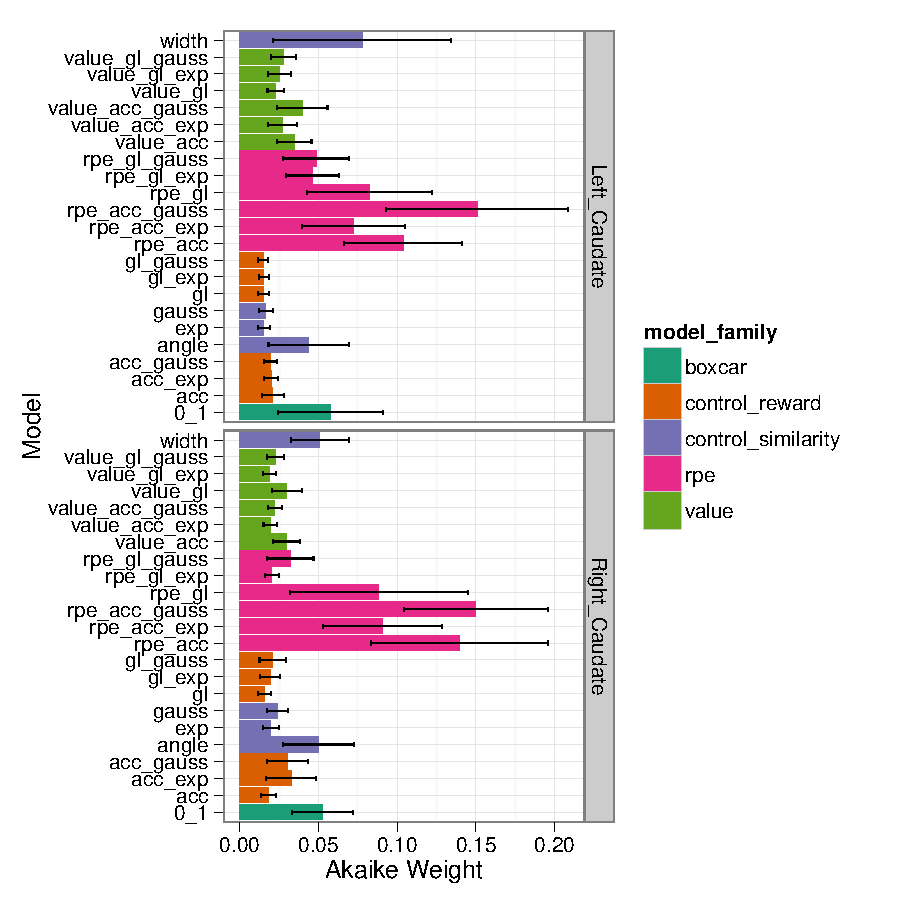
\includegraphics[width=39pc]{f_meanbar_run4_c_aic_w_bilat_Caudate}
    \centering
    \caption{Dorsal caudate (left and right) -- Akaike Weights for all models.  Colors indicate model family (see p\pageref{sub:cmb} for details). Bars represent standard errors.}
    \label{fig:caudate}
\end{figure}
\begin{figure}[tp]
    \noindent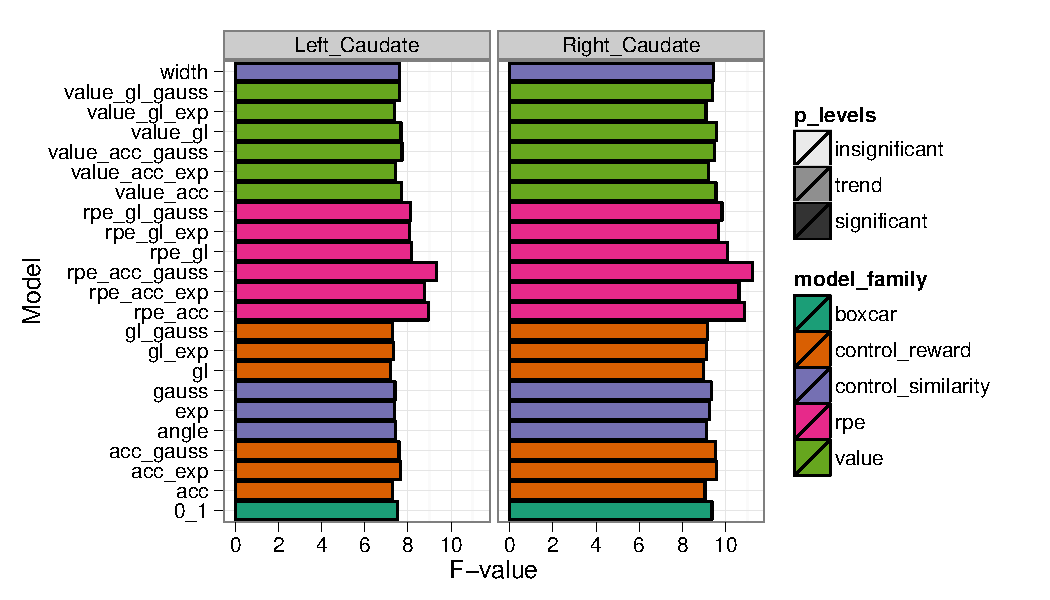
\includegraphics[width=39pc]{f_plot_run4_c_fvalue_bilat_Caudate}
    \centering
    \caption{Dorsal caudate (left and right) -- $F$-values for all models.  Significance-level is denoted by the saturation, where the $p <$ 0.05 level is significant, and trend is between $p <$ 0.05 and 0.10.  Colors indicate model family (see p\pageref{sub:cmb} for details).}
    \label{fig:fvalcaudate}
\end{figure}

\begin{figure}[tp]
    \noindent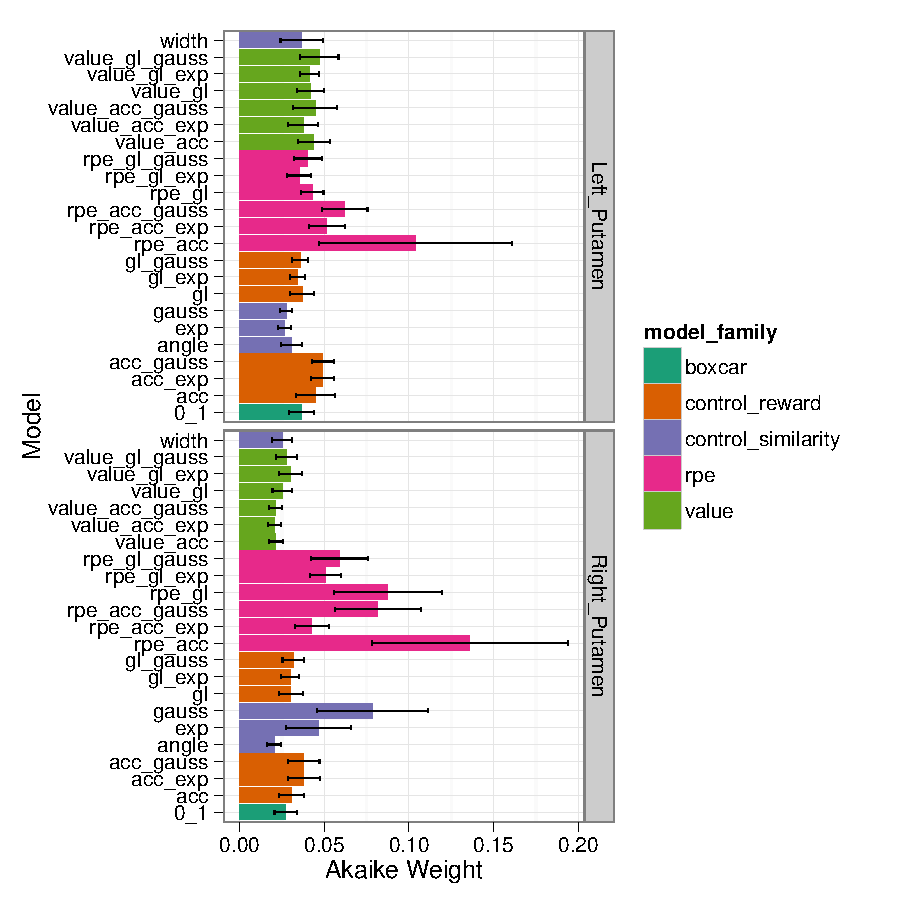
\includegraphics[width=39pc]{f_meanbar_run4_c_aic_w_bilat_Putamen}
    \centering
    \caption{Putamen (left and right) -- Akaike Weights for all models.  Colors indicate model family (see p\pageref{sub:cmb} for details). Bars represent standard errors.}
    \label{fig:putamen}
\end{figure}
\begin{figure}[tp]
    \noindent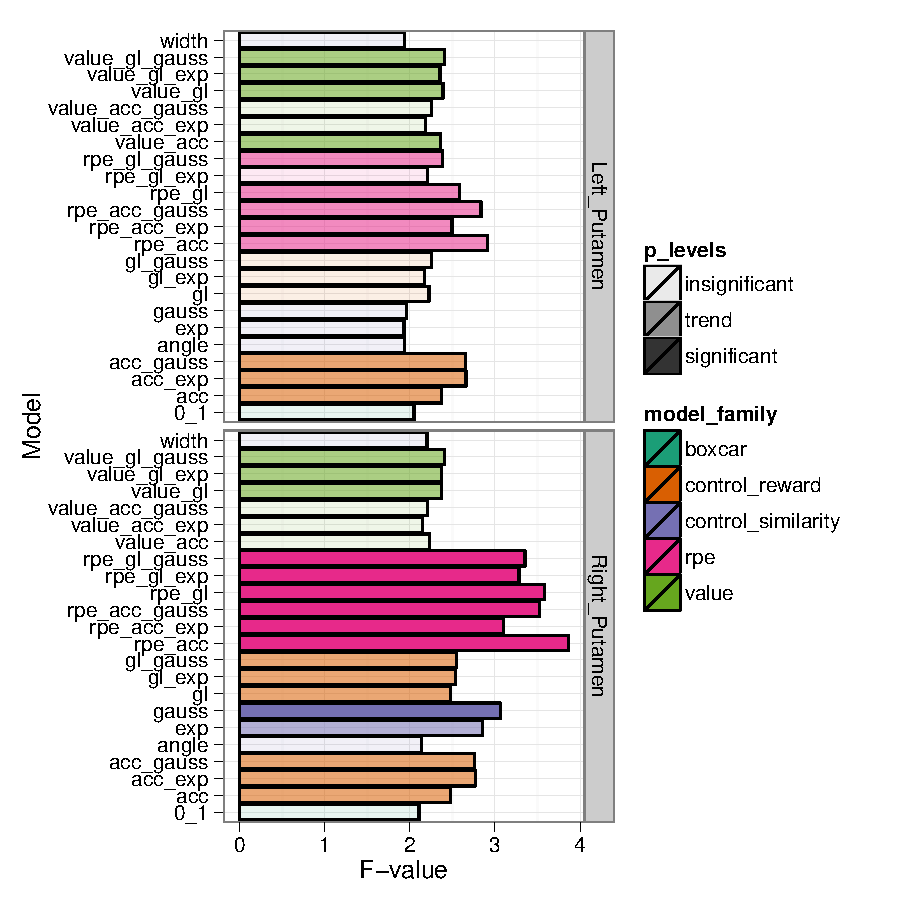
\includegraphics[width=39pc]{f_plot_run4_c_fvalue_bilat_Putamen}
    \centering
    \caption{Putamen (left and right) -- $F$-values for all models.
    Significance-level is denoted by the saturation, where the $p <$ 0.05 level is
    significant, and trend is between $p <$ 0.05 and 0.10.  Colors indicate model family (see p\pageref{sub:cmb} for details).}
    \label{fig:fvalputamen}
\end{figure}


\begin{figure}[tp]
    \noindent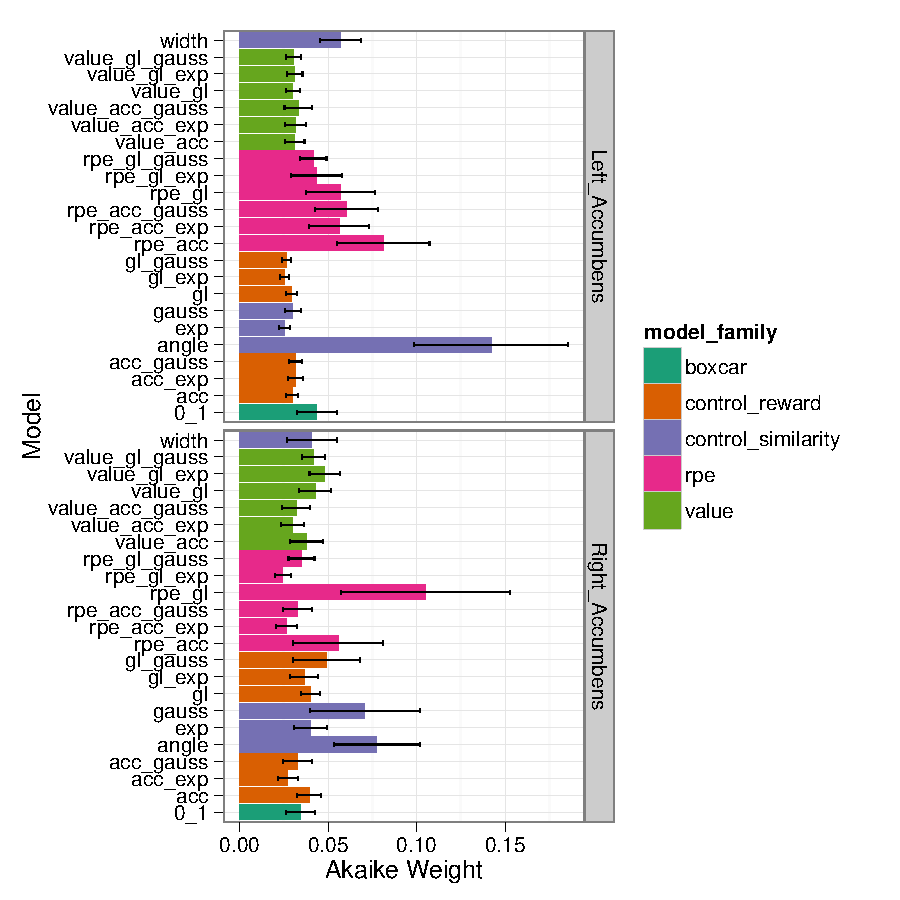
\includegraphics[width=39pc]{f_meanbar_run4_c_aic_w_bilat_Accumbens}
    \centering
    \caption{Nucleus Accumbens (left and right) -- Akaike Weights for all models.  Colors indicate model family (see p\pageref{sub:cmb} for details). Bars represent standard errors.}
    \label{fig:accumbens}
\end{figure}
\begin{figure}[tp]
    \noindent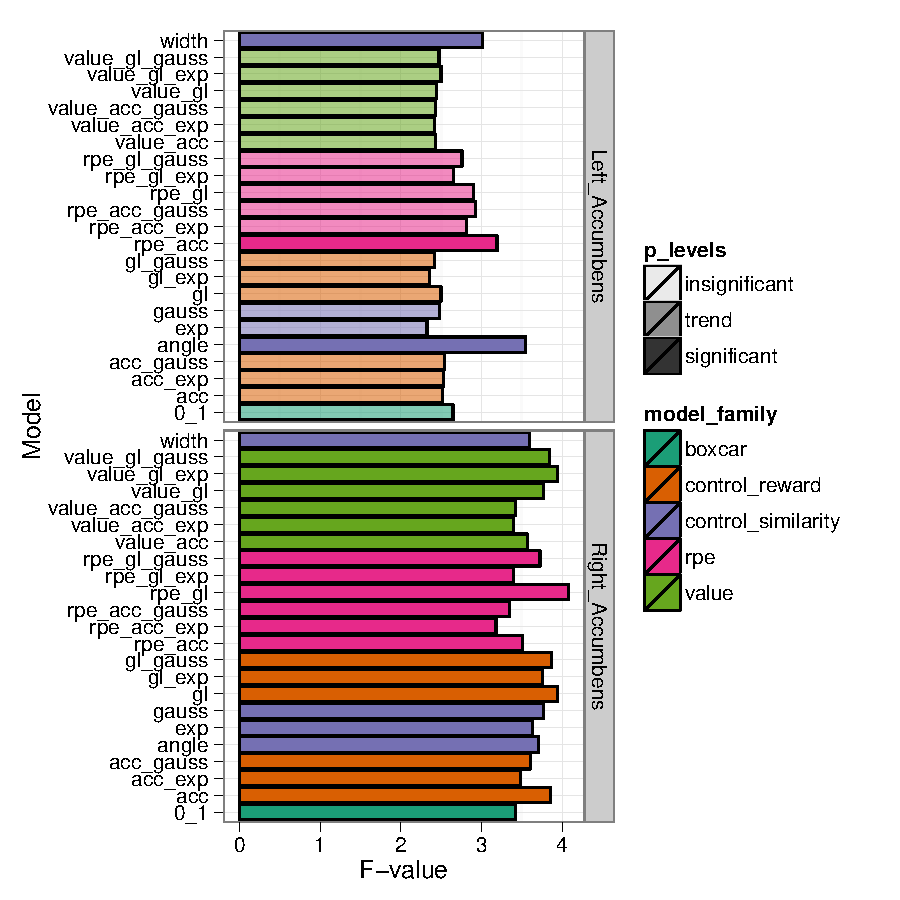
\includegraphics[width=39pc]{f_plot_run4_c_fvalue_bilat_Accumbens}
    \centering
    \caption{Nucleus accumbens (left and right) -- $F$-values for all models.
    Significance-level is denoted by the saturation, where the $p <$ 0.05 level is
    significant, and trend is between $p <$ 0.05 and 0.10.  Colors indicate model family (see p\pageref{sub:cmb} for details).}
    \label{fig:fvalaccumbens}
\end{figure}

\subsubsection{On that thinking sheet}
\label{subsub:onsheet}
The insula was the one region, both cortically and subcortically, to be nearly equally well described both by the ``acc'' and ``gl'' reward codes (Figure~\ref{fig:insula}).  In the top ranking ``rpe'' family (which was 1.37 times more likely than its neighbor ``control\_similarity'', and 2.31 more likely than the ``boxcar'') within-family models showed divergent patterns based on the code.  The ``acc'', ``rpe\_acc'' and ``rpe\_acc\_gauss'' models dominated ``rpe\_acc\_exp'' (around 1.4).  The ``gl'' code had the opposite effect, ``rpe\_gl\_exp'' dominated ``rpe\_gl'' and ``rpe\_gl\_gauss'' by a somewhat similar amount (1.20).  The strong overall significance of all models (Figure~\ref{fig:fvalinsula}) suggests these relative rankings may reflect truth; like the dorsal caudate the $F$-values the have same patterns as Akaike Weights.

Both the ACC and PCC displayed very similar rankings of their Akaike Weights (compare Figures~\ref{fig:ant} to~\ref{fig:post}), so they'll be discussed as one.  Again the ``rpe'' family dominated (respectively 2.07 and 1.77 times more likely compared to the nearest neighbor, 2.86 and 2.88 times more likely then the ``boxcar'').  Unlike the caudate and insula, the 2 similarity-adjustment models (``rpe\_acc\_gauss'' and ``rpe\_acc\_exp'') were consistently more informative than the reward unadjusted (``rpe\_acc'').  Looking at the $F$-tests, both regions, especially in the ``rpe'' family were reasonably significant (Figure~\ref{fig:fvalant} and~\ref{fig:fvalpost}).

Like the orbital frontal (below), ``boxcar'' was the most informative family for the middle frontal cortex (Figure~\ref{fig:dlpfc}), however model-wise ``rpe\_acc'' was 2.07 times more likely.  The strong $F$-values for all models, and ``rpe\_acc'' especially (the largest observed for all models and regions; Figure~\ref{fig:fvaldlpfc}), lend strong support then for selecting ``rpe\_acc'' as the sole best explanation of this regions activity.

Both the frontal medial (ventrolateral) and orbital frontal results are difficult to interpret, but for different reasons.  Nearly all families, and models, in frontal medial cortex ranked as substantively more likely that the ``boxcar'' (ranging, at the family level, from 2.13 for ``control\_similarity'' to 1.75 for ``value'', with higher scores for individual models).  However none of the models were substantively (or even slightly) more likely than any of their neighbors.  So while, as measured by the $F$-tests, there was significant activity in medial frontal (Figure~\ref{fig:fvalvmpfc}) it is not well accounted for by any of the candidate models.  Orbital frontal cortex though has the opposite problem.  The ``boxcar'' had the largest Akaike Weight (Figure~\ref{fig:ofc}).  However at the model-level ``rpe\_acc\_gauss'' and ``rpe\_acc'' both score slightly better (1.32 and 1.34, respectively).  However these slight increase are weak evidence when the alternative is that nothing has changed from trial-to-trial (i.e., the ``boxcar'' model).  Additionally as ACC and OFC are tightly functionally interconnected \citep{Rudebeck:2008p4712}, these weak likelihoods may be carryover from the strong ``rpe'' signals observed in the ACC (Figure~\ref{fig:ant}).

\begin{figure}[tp]
    \noindent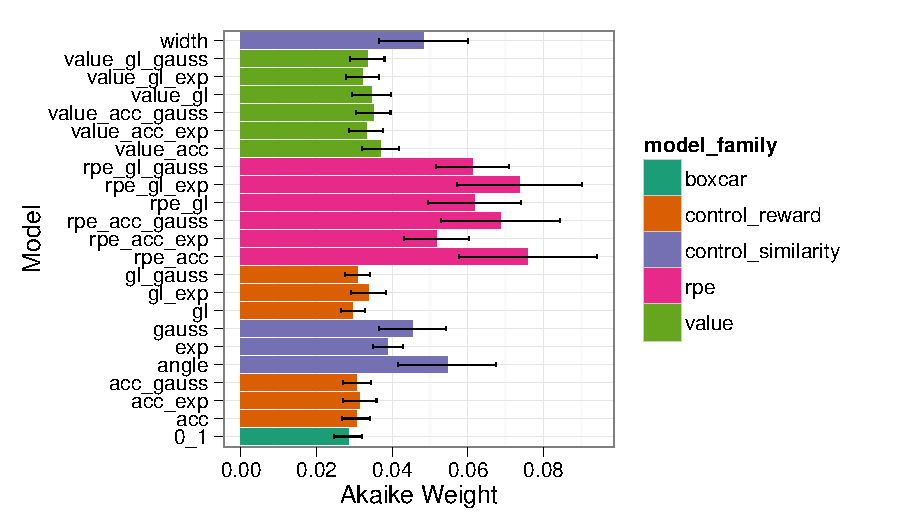
\includegraphics[width=39pc]{f_meanbar_run4_c_aic_w_Insular_Cortex}
    \centering
    \caption{Bilateral Insula -- Akaike Weights for all models.  Colors indicate model family (see p\pageref{sub:cmb} for details). Bars represent standard errors.}
    \label{fig:insula}
\end{figure}
\begin{figure}[tp]
    \noindent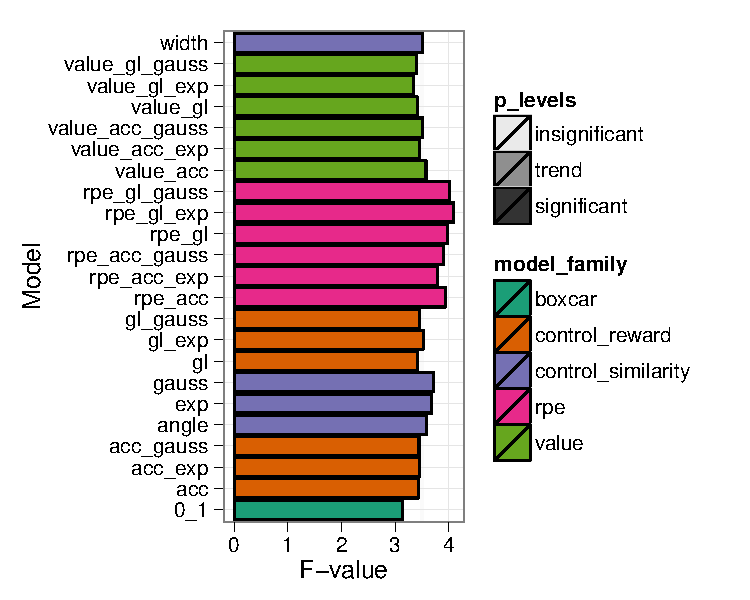
\includegraphics[width=39pc]{f_plot_run4_c_fvalue_Insular_Cortex}
    \centering
    \caption{Bilateral Insula -- $F$-values for all models.
    Significance-level is denoted by the saturation, where the $p <$ 0.05 level is
    significant, and trend is between $p <$ 0.05 and 0.10.  Colors indicate model family (see p\pageref{sub:cmb} for details).}
    \label{fig:fvalinsula}
\end{figure}


\begin{figure}[tp]
    \noindent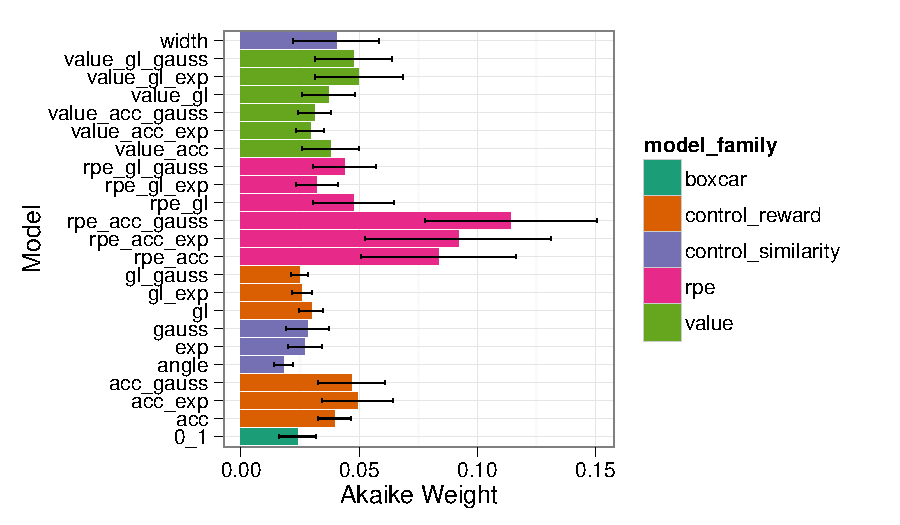
\includegraphics[width=39pc]{f_meanbar_run4_c_aic_w_Cingulate_Gyrus_anterior_division}
    \centering
    \caption{ACC -- Akaike Weights for all models.  Colors indicate model family (see p\pageref{sub:cmb} for details). Bars represent standard errors.}
    \label{fig:ant}
\end{figure}
\begin{figure}[tp]
    \noindent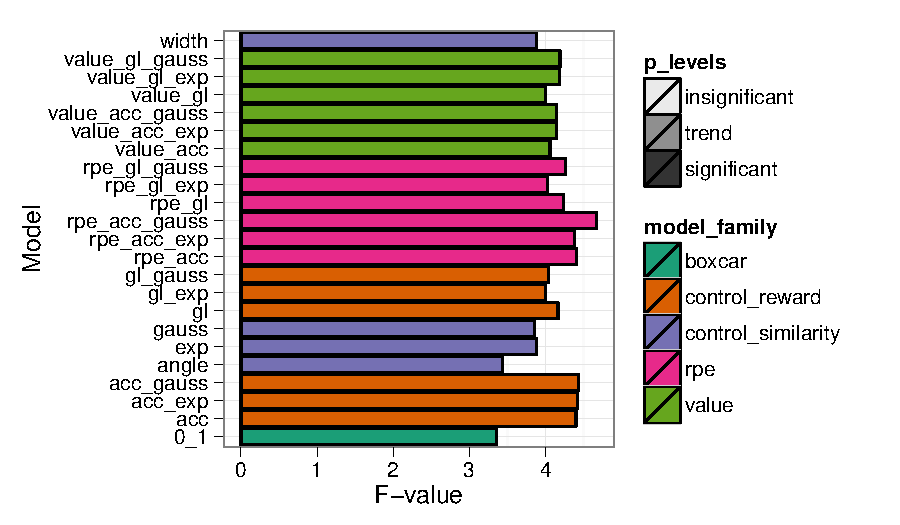
\includegraphics[width=39pc]{f_plot_run4_c_fvalue_Cingulate_Gyrus_anterior_division}
    \centering
    \caption{ACC -- $F$-values for all models.
    Significance-level is denoted by the saturation, where the $p <$ 0.05 level is
    significant, and trend is between $p <$ 0.05 and 0.10.  Colors indicate model family (see p\pageref{sub:cmb} for details).}
    \label{fig:fvalant}
\end{figure}


\begin{figure}[tp]
    \noindent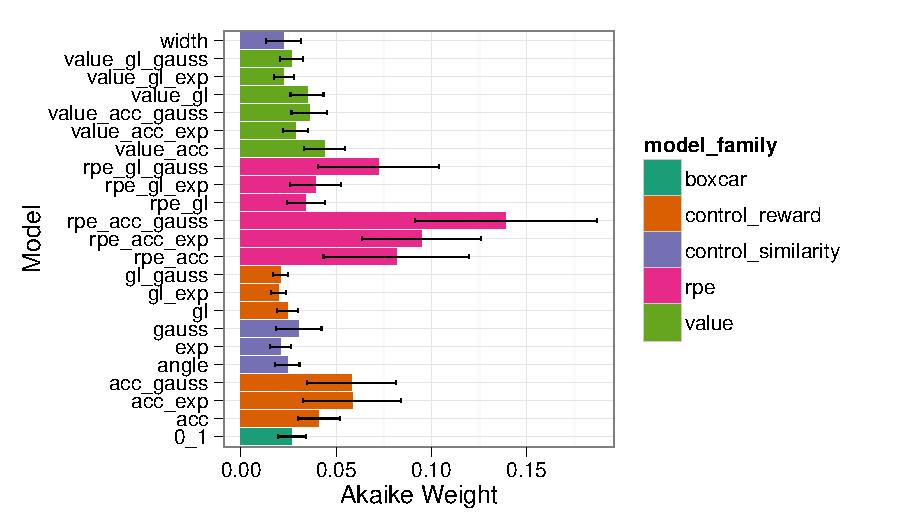
\includegraphics[width=39pc]{f_meanbar_run4_c_aic_w_Cingulate_Gyrus_posterior_division}
    \centering
    \caption{PCC -- Akaike Weights for all models.  Colors indicate model family (see p\pageref{sub:cmb} for details). Bars represent standard errors.}
    \label{fig:post}
\end{figure}
\begin{figure}[tp]
    \noindent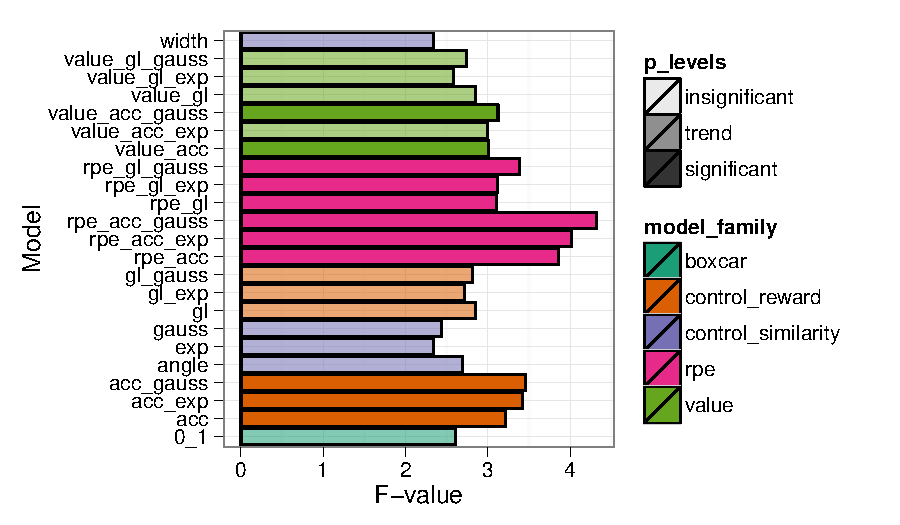
\includegraphics[width=39pc]{f_plot_run4_c_fvalue_Cingulate_Gyrus_posterior_division}
    \centering
    \caption{PCC -- $F$-values for all models.
    Significance-level is denoted by the saturation, where the $p <$ 0.05 level is
    significant, and trend is between $p <$ 0.05 and 0.10.  Colors indicate model family (see p\pageref{sub:cmb} for details).}
    \label{fig:fvalpost}
\end{figure}

\begin{figure}[tp]
    \noindent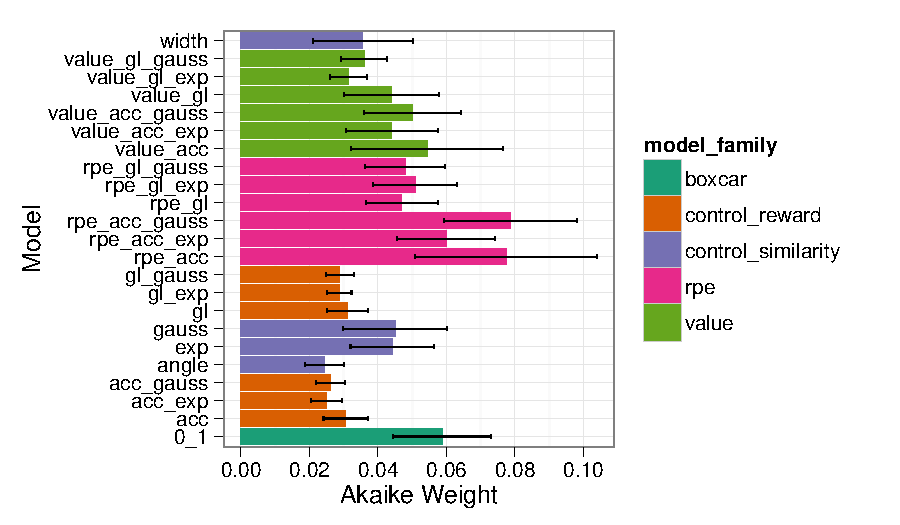
\includegraphics[width=39pc]{f_meanbar_run4_c_aic_w_Frontal_Orbital_Cortex}
    \centering
    \caption{Orbital frontal cortex -- Akaike Weights for all models.  Colors indicate model family (see p\pageref{sub:cmb} for details). Bars represent standard errors.}
    \label{fig:ofc}
\end{figure}
\begin{figure}[tp]
    \noindent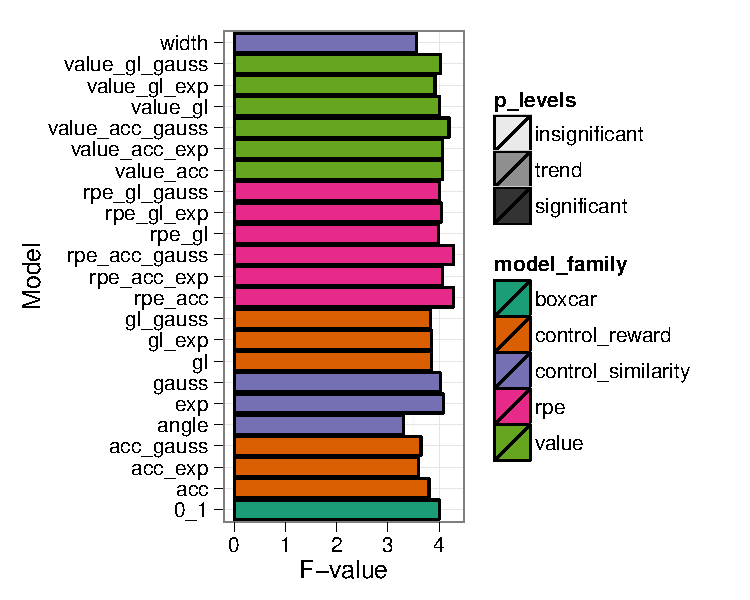
\includegraphics[width=39pc]{f_plot_run4_c_fvalue_Frontal_Orbital_Cortex}
    \centering
    \caption{Orbital frontal cortex -- $F$-values for all models.
    Significance-level is denoted by the saturation, where the $p <$ 0.05 level is
    significant, and trend is between $p <$ 0.05 and 0.10.  Colors indicate model family (see p\pageref{sub:cmb} for details).}
    \label{fig:fvalofc}
\end{figure}


\begin{figure}[tp]
    \noindent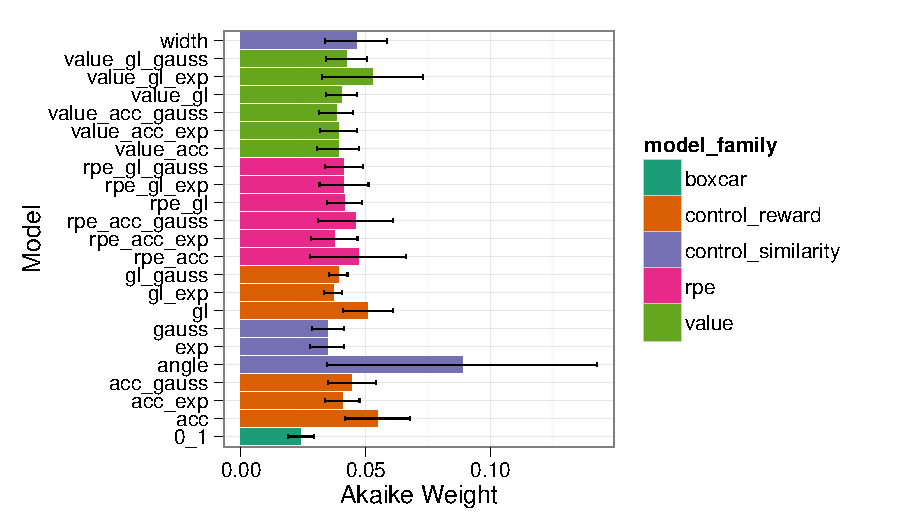
\includegraphics[width=39pc]{f_meanbar_run4_c_aic_w_Frontal_Medial_Cortex}
    \centering
    \caption{Frontal (ventral)medial PFC -- Akaike Weights for all models.  Colors indicate model family (see p\pageref{sub:cmb} for details). Bars represent standard errors.}
    \label{fig:vmpfc}
\end{figure}
\begin{figure}[tp]
    \noindent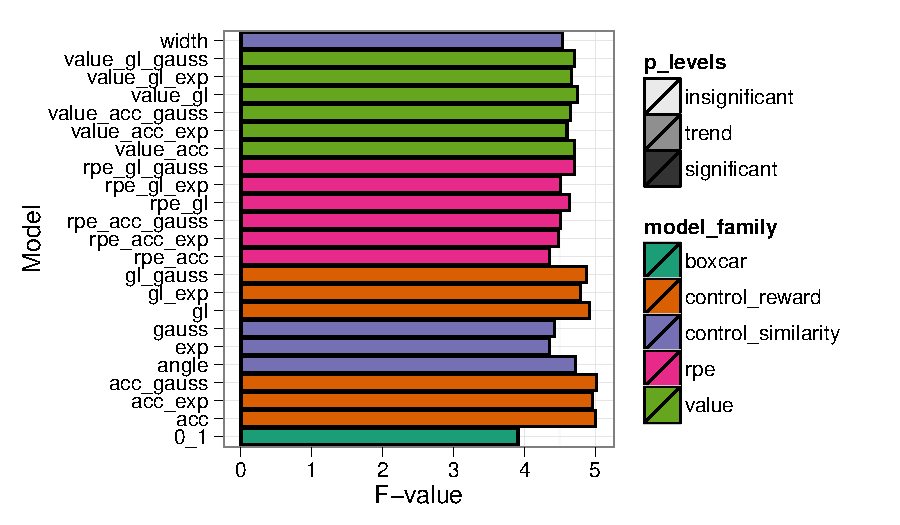
\includegraphics[width=39pc]{f_plot_run4_c_fvalue_Frontal_Medial_Cortex}
    \centering
    \caption{Frontal (ventral)medial PFC -- $F$-values for all models.
    Significance-level is denoted by the saturation, where the $p <$ 0.05 level is
    significant, and trend is between $p <$ 0.05 and 0.10.  Colors indicate model family (see p\pageref{sub:cmb} for details).}
    \label{fig:fvalvmpfc}
\end{figure}

\begin{figure}[tp]
    \noindent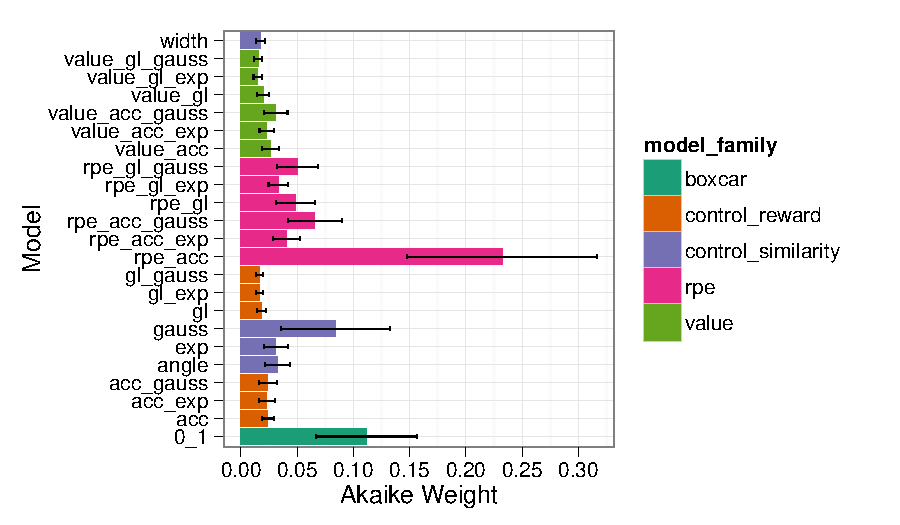
\includegraphics[width=39pc]{f_meanbar_run4_c_aic_w_Middle_Frontal_Gyrus}
    \centering
    \caption{Middle frontal (dorsolateral) PFC -- Akaike Weights for all models.  Colors indicate model family (see p\pageref{sub:cmb} for details). Bars represent standard errors.}
    \label{fig:dlpfc}
\end{figure}
\begin{figure}[tp]
    \noindent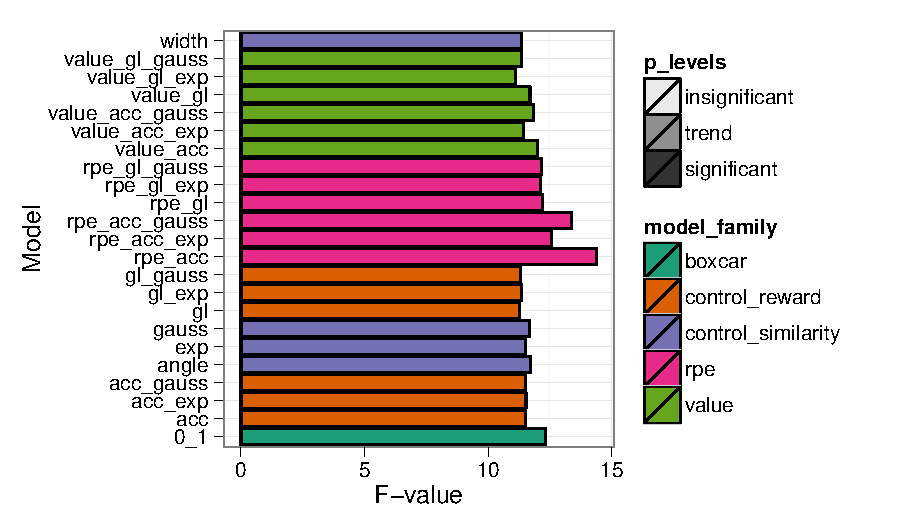
\includegraphics[width=39pc]{f_plot_run4_c_fvalue_Middle_Frontal_Gyrus}
    \centering
    \caption{Middle frontal (dorsolateral) PFC -- $F$-values for all models.
    Significance-level is denoted by the saturation, where the $p <$ 0.05 level is
    significant, and trend is between $p <$ 0.05 and 0.10.  Colors indicate model family (see p\pageref{sub:cmb} for details).}
    \label{fig:fvaldlpfc}
\end{figure}
\clearpage